\documentclass[11pt]{exam}
\usepackage[utf8]{inputenc}
\usepackage[a4paper,top=2cm,left=2cm,right=2cm,bottom=2cm]{geometry}
\usepackage{import}
\usepackage[T1]{fontenc}
\usepackage[german,ngerman]{babel}
\usepackage[table]{xcolor}
\usepackage{amsthm, esvect}
\usepackage{mathtools}
\RequirePackage{amssymb, amsfonts, amsmath, latexsym, verbatim, xspace}
\usepackage{systeme}
\usepackage{multicol}
\usepackage{multirow}
\usepackage{framed}
\usepackage{array}
\usepackage{ragged2e}
\usepackage{graphicx}
\usepackage{pdflscape}
\usepackage{epstopdf}
\usepackage{booktabs}
\usepackage{pdfpages}
\usepackage{float} % Allows putting an [H] in \begin{figure} to specify the exact location of the figure
\usepackage{wrapfig} % Allows in-line images such as the example fish picture
\usepackage{tikz, graphicx} % tikz
\usepackage[position=top]{subfig}
\usepackage[bookmarks=true]{hyperref}%Links
\usepackage{enumerate}
\usepackage{enumitem}
\usepackage[german,ruled,vlined,linesnumbered,algosection]{algorithm2e}
\usepackage[labelfont=sf]{caption}
\usepackage{lmodern}
\usepackage{lscape}
\usepackage{tabularx}
\usepackage{systeme}
\usepackage{hhline}
\usepackage{subfiles}
\usepackage{stackengine}
\usepackage{setspace}
\usepackage{MnSymbol}
\usepackage{tcolorbox}
\usepackage{bbm}
\usepackage{url}
\usepackage{xparse}
\usepackage{sectsty}
\usepackage{array}
\usepackage{ragged2e}
\usepackage{listings} %Stellt Code-Snippets sauber dar

% definiert die Sprache
\selectlanguage{German}

% add command for different dates in Swiss fashion
\newcommand{\monthwordlong}[1]{\ifcase#1 \or Januar\or Februar\or März\or April\or Mai\or Juni\or Juli\or August\or September\or Oktober\or November\or Dezember\fi}
\newcommand{\monthwordshort}[1]{\ifcase#1\or Jan\or Feb\or Mar\or Apr\or Mai\or Jun\or Jul\or Aug\or Sept\or Okt\or Nov\or Dez\fi}
\newcommand{\datelong}{\number\day.\:\monthwordlong{\the\month}\:\number\year}
\newcommand{\dateshort}{\number\day.\:\monthwordshort{\the\month}\:\number\year}

% define color of links inside a text
\definecolor{linkblue}{RGB}{0, 0, 80}
\definecolor{plotblue}{RGB}{100, 100, 255}
\definecolor{myblue}{RGB}{8,164,214}
\definecolor{myred}{RGB}{143,42,41}
\definecolor{forestgreen}{RGB}{34,139,34}
\definecolor{highdive}{RGB}{10,169,194}
\definecolor{charcoal}{RGB}{74,74,74}
\hypersetup{
	colorlinks=true,
	linkcolor=linkblue,
	filecolor=magenta,
	urlcolor=plotblue,
	citecolor=linkblue,
	pdfpagemode=FullScreen,
}


\lstdefinestyle{mystyle}{ % definiert den style des Code-Snippets
	%backgroundcolor=\color{backcolour},
	%commentstyle=\color{codegreen},
	%keywordstyle=\color{magenta},
	%numberstyle=\tiny\color{codegray},
	%stringstyle=\color{codepurple},
	basicstyle=\ttfamily\footnotesize,
	breakatwhitespace=false,
	breaklines=true,
	captionpos=b,
	keepspaces=true,
	%numbers=left,
	%numbersep=5pt,
	showspaces=false,
	showstringspaces=false,
	showtabs=false,
	tabsize=4
}
\lstset{style=mystyle}
\qformat{\Large\textbf{Aufgabe \thequestion\hfill\thepoints}}
\newlist{partes}{enumerate}{3}
\setlist[partes]{label=(\alph*)}
\newcommand{\parte}{\item}
\newlist{subpartes}{enumerate}{3}
\setlist[subpartes]{label=\roman*)}
\newcommand{\subparte}{\item}
\setlist[enumerate,1]{%(
	leftmargin=*, itemsep=12pt, label={\textbf{\arabic*.)}}}
\newcommand\answerbox{%%
	\fbox{\rule{2in}{0pt}\rule[-0.1ex]{0pt}{4ex}}}
\pointpoints{Punkt}{Punkte}
\hqword{Frage:}
\hpword{Mögliche Punkte:}
\hsword{Erreicht:}
\htword{Total}
\renewcommand*\half{.5}
\renewcommand{\solutiontitle}{\noindent\textbf{Lösung:}\par\noindent}

% Graphed boxes
\newcommand{\karos}[2]{
  \begin{tikzpicture}
    \draw[step=0.4cm,color=cyan,dotted] (0,0) grid (#1 cm ,#2 cm);
  %  \draw((#1)/2 cm,0)--((#1)/2 cm,/#2)/2cm)
  \end{tikzpicture}
}
\usetikzlibrary{arrows, petri, topaths, graphs}
\linespread{1.2} % Line spacing

%=========================================================
\newenvironment{parcols}[1][]{
    \begin{parts}\begin{multicols}{#1}
}{
    \end{multicols}\end{parts}
}
%=========================================================
\newenvironment{itemcols}[1][]{
	\begin{itemize}\begin{multicols}{#1}
		}{
	\end{multicols}\end{itemize}
}

%=========================================================
\newcommand{\antwort}[1]{
	{\setlength{\textwidth}{\textwidth}\fillwithgrid{#1cm}\vspace{5pt}}
}

%=========================================================
% Karriertes Papier für Antwort MIT OVERLAY
\tcbuselibrary{breakable,skins}
\usetikzlibrary{mindmap,trees}
\newlength\tindent
\setlength{\tindent}{\parindent}
\setlength{\parindent}{0pt}
\setlength{\parskip}{0pt}

\newtcolorbox{gridspace}[1]{%
	enhanced,
	breakable,
	blanker,
	boxrule=0pt,
	left=5mm,
	right=5mm,
	top=5.75mm,
	bottom=0mm,
	boxsep=0pt,
	height=#1cm,
	width=16cm,
	before upper={
		\begingroup
		\setlength{\baselineskip}{5.75mm}
		\setlength{\parskip}{0pt}
		\setlength{\lineskip}{0pt}
		% keep every paragraph on the grid rhythm
		%\everypar{\vspace{0pt}\strut}
		% math formulas shifted by one grid row
		\let\oldbracketopen\[
		\renewcommand{\[}{\vspace{-5mm}\oldbracketopen}
		% Align displayed formulas to the grid
		\setlength{\abovedisplayskip}{0pt}
		\setlength{\belowdisplayskip}{0pt}
		\setlength{\abovedisplayshortskip}{0pt}
		\setlength{\belowdisplayshortskip}{0pt}
		% Enumerate follows the same rhythm
		\setlist[enumerate]{leftmargin=6mm,itemsep=0mm,topsep=0pt,parsep=0pt,partopsep=0pt}
		\setlist[itemize]{leftmargin=6mm,itemsep=10mm,topsep=0pt,parsep=0pt,partopsep=0pt}},
	after upper={
		\endgroup},
	underlay={
		\draw[step=5mm,color=gray!55] (interior.south west) grid (interior.north east);}
}

%%
% Math Arrows
%%
\newcommand{\same}{\ensuremath{\Longleftrightarrow}}
\renewcommand{\to}{\ensuremath{\longrightarrow}}
\newcommand{\qsame}{\quad\same\quad}
\newcommand{\dsame}{\ensuremath{:\Leftrightarrow}}
\newcommand{\qdsame}{\quad\dsame\quad}
\newcommand{\ldsame}{\ensuremath{:\Longleftrightarrow}}
\newcommand{\samedef}{\ensuremath{\us {\text{def}} \Leftrightarrow}}
\newcommand{\qsamedef}{\quad\samedef\quad}
\newcommand{\lsamedef}{\ensuremath{\us {\text{def}} \Longleftrightarrow}}
\newcommand{\qlsamedef}{\quad\lsamedef\quad}


%%
% Mengendefinitionen
%%
\newcommand{\M}{\ensuremath{\mathcal{M}}}
\newcommand{\N}{\ensuremath{\mathbb{N}}}
\newcommand{\Z}{\ensuremath{\mathbb{Z}}}
\newcommand{\Q}{\ensuremath{\mathbb{Q}}}
\newcommand{\I}{\ensuremath{\mathbb{I}}}
\newcommand{\R}{\ensuremath{\mathbb{R}}}
\newcommand{\C}{\ensuremath{\mathbb{C}}}
\renewcommand{\S}{\ensuremath{\mathbb{S}}}
\newcommand{\Prim}{\ensuremath{\mathbb{P}}}
\newcommand{\0}{\ensuremath{\emptyset}}
\renewcommand{\Re}{\ensuremath{\operatorname{Re}}}
\renewcommand{\Im}{\ensuremath{\operatorname{Im}}}
\newcommand{\strich}{\ensuremath{\big\vert}}

%%
% Mengenoperation
%%
\renewcommand{\nin}{\not\in}


%%
% Logisches Und und Oder
%%
\newcommand{\sand}{\ensuremath{\; \land \;}}
\newcommand{\sor}{\ensuremath{\; \lor \;}}
\renewcommand{\*}{\ensuremath{\cdot}}
\newcommand{\oder}{\vee}
\newcommand{\n}{\neg}
\newcommand{\und}{\wedge}


%%
% Bei Integral, Summe,... die Grenzen über bzw.
% unter das Zeichen
%%
\renewcommand{\d}[1]{\ensuremath{\operatorname{d}\!{#1}}}
\newcommand{\Sum}{\sum\limits}
\newcommand{\Prod}{\prod\limits}
\newcommand{\Min}{\min\limits}
\newcommand{\Max}{\max\limits}
\newcommand{\Lim}{\lim\limits}
\newcommand{\Inf}{\inf\limits}
\newcommand{\Sup}{\sup\limits}
\newcommand{\Liminf}{\liminf\limits}
\newcommand{\Limsup}{\limsup\limits}
%\renewcommand{\Cup}{\bigcup\limits}
%\renewcommand{\Cap}{\bigcap\limits}
\newcommand{\Otimes}{\bigotimes\limits}
\newcommand{\Oplus}{\bigoplus\limits}


%%
% Arcus Cotangens, Logarithmus
%%
\let\oldsin\sin
\renewcommand{\sin}[1]{\oldsin{\left(#1\right)}}
\let\oldcos\cos
\renewcommand{\cos}[1]{\oldcos{\left(#1\right)}}
\let\oldtan\tan
\renewcommand{\tan}[1]{\oldtan{\left(#1\right)}}
\let\oldarcsin\arcsin
\renewcommand{\arcsin}[1]{\oldarcsin{\left(#1\right)}}
\let\oldarccos\arccos
\renewcommand{\arccos}[1]{\oldarccos{\left(#1\right)}}
\let\oldarctan\arctan
\renewcommand{\arctan}[1]{\oldarctan{\left(#1\right)}}
\let\oldln\ln
\renewcommand{\ln}[1]{\oldln{\left(#1\right)}}
\newcommand{\Log}[2]{\ensuremath{\operatorname{log}_{#1}\left(#2\right)}}
\newcommand{\e}{\operatorname{e}}
\renewcommand{\exp}[1]{\ensuremath{\operatorname{\e}^{#1}}}


%%
% Griechische Buchstaben
%%
\renewcommand{\epsilon}{\ensuremath{\varepsilon}}
\renewcommand{\phi}{\varphi}
\renewcommand{\l}{\lambda}
\renewcommand{\t}{\tau}


%%
% Bezeichnungen
%%
\newcommand{\Rgn}{\R_{>0}} % R grösser Null
\newcommand{\Rad}{\operatorname{Rad}}   % Radikal
\newcommand{\kgV}{\operatorname{kgV}}   % Kleinster gemeinsame Vielfache
\newcommand{\ggT}{\operatorname{ggT}}   % Grösster gemeinsame Teiler
\newcommand{\winkel}{\sphericalangle}          % Winkelsymbol
\DeclarePairedDelimiter\abs{\lvert}{\rvert} % besserer Betrag
\makeatletter
\let\oldabs\abs
\def\abs{\@ifstar{\oldabs}{\oldabs*}}
\makeatother


%%
% Vektorgeometrie
%%
\renewcommand{\v}[1]{\vv{#1}}       % besserer Pfeil über Buchstaben
\renewcommand{\vec}[2]{\begingroup\renewcommand{\arraystretch}{1}\left(\begin{array}{c} #1 \\ #2 \end{array}\right)\endgroup}   % two dimensional vector
\renewcommand{\Vec}[3]{\begingroup\renewcommand{\arraystretch}{1}\left(\begin{array}{c} #1 \\ #2 \\ #3 \end{array}\right)\endgroup}      % three dimensional vector


%%
% Text
%%
\newcommand*{\Ueq}[1]{\mathrel{\mathop{=}\limits_{\text{#1}}}}
\newcommand*{\Oeq}[1]{\mathrel{\stackrel{\text{#1}}{=}}}
\newcommand{\utext}[2]{\underbrace{#1}_{\substack{#2}}}
\newcommand{\otext}[2]{$\overbrace{\textrm{#1}}^{\textrm{#2}}$}
\newcommand{\lineortext}[1]{\hspace{0,1cm}\underline{\hspace{0.1cm}\hphantom{#1}\hspace{0.1cm}}\hspace{0,1cm}} % Lückentext erstellen
\newcommand{\gap}[1]{\rule{#1 cm}{1pt}}
\pagestyle{headandfoot}
\firstpageheader{}{}{}
\runningheader{\date}{}{\class, \teacher}
\runningheadrule
\firstpagefooter{}{}{}
\runningfooter{}{Viel Erfolg!}{Seite \thepage\:von \numpages}
\runningfootrule
%=========================================================
\newcommand{\theme}{Folgen, Reihen und Grenzwerte}
\newcommand{\teacher}{Jonas Guler}
\newcommand{\class}{3Na}
\renewcommand{\date}{27.03.25}
%=========================================================
\begin{document}
\fontsize{14}{14}\selectfont
%========================================================
\noindent
\begingroup
\renewcommand{\arraystretch}{1.5}
\begin{tabular*}{\textwidth}{l @{\extracolsep{6pt}}l @{\extracolsep{\fill}}l @{\extracolsep{6pt}}l}
	\multicolumn{2}{l}{{\bf \theme}} & {\bf Note:} & {\answerbox}\\
	\multicolumn{2}{l}{{\bf \teacher}} & & \\
	{\bf Klasse:} & {\class} &  {\bf Name:} &\textbf{\hrulefill}\\
	{\bf Dauer:} & $45$ Minuten & {\bf Datum:} & {\date}\\[8pt]
\end{tabular*}
\endgroup
\rule[1ex]{\textwidth}{1pt}
%=========================================================
\begin{center}
    \textbf{Bewertungstabelle}\\
    \small Wird von der Lehrperson ausgefüllt\\
    \vspace{5pt}
    \addpoints
    \gradetable[h][questions]\\
    \vspace{5pt}
    Der Rechenweg muss \textbf{vollständig und nachvollziehbar} sein.\\
    Lösen Sie die Prüfung mit einen schwarzen oder blauen Kugelschreiber.\\
    Als Hilfsmittel ist nur der Taschenrechner erlaubt.\\
\end{center}
\rule[1ex]{\textwidth}{1pt}

\vspace{10cm}
\begin{center}
    %\Huge{Repetitionsprüfung}
\end{center}

\newpage
\begin{questions}
%=========================================================
%-------------------TESTFRAGEN
%=========================================================
\noaddpoints
\question[\totalpoints]
\addpoints
\begin{parts}
    \part[3] Erkläre einem Laien unter welchen Bedingungen eine unendliche geometrische Reihe konvergiert. Erfinde dazu passende Beispiele.
\end{parts}
\vspace{5pt}
\antwort{10}
\begin{parts}
    \setcounter{partno}{1}
    \part[2] Von einer geometrischen Folge sind zwei Folgenglieder bekannt, $a_2=96$ und $a_9=1640.25$. Berechne $q$ und $a_{35}$.
\end{parts}
\vspace{5pt}
\antwort{11}
\newpage

%---------------------------------------------------------
\question[3] %DMK Ana S29 A180
Von einer geometrischen Folge sind $a_7=\frac{729}{32}$ und $q=\frac{3}{4}$ bekannt. Berechne den Grenzwert $s$ der unendlichen geometrischen Reihe.
\vspace{5pt}
\antwort{10.5}
\question[3] % DMK Ana S29 A183a
Berechne den Grenzwert der folgenden Summe: \[16+12+9+\ldots=\]
\antwort{10}

%---------------------------------------------------------
\newpage
\noaddpoints
\question[\totalpoints] %DMK Ana S29 A182
\addpoints
\begin{minipage}{0.6\linewidth}
	Gegeben ist ein Quadrat mit Seitenlänge 100 cm, in welches weitere Quadrate einbeschrieben sind (siehe Skizze). $Q_1,Q_2,Q_3,\ldots$ ist die Folge der Flächeninhalte der einbeschriebenen Quadrate, deren Seitenlänge eine Geometrische Folge bilden.
\end{minipage}
\hfill
\begin{minipage}{0.35\linewidth}
	\centering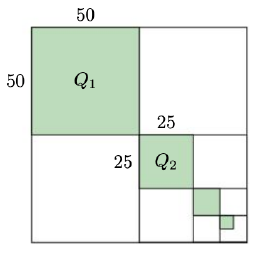
\includegraphics[scale=0.6]{Analysis/data-analysis/FR_Quadrate.png}
\end{minipage}
\begin{parts}
	\part[2] Bestimme die explizite Beschreibung für die Folge der Flächeninhalte $Q_n$.
	\part[2] Ab welchem $n\in\N$ ist der Flächeninhalt $Q_n$ kleiner als $10^{-34}$?
	\part[2] Bestimme die Gesamtfläche der ersten $10$ Quadrate.
	\part[2] Gegen welchen Wert strebt die Summe der Flächeninhalte aller Quadrate?
\end{parts}
\vspace{5pt}
\antwort{17}

%---------------------------------------------------------
\newpage
\question[4]
Begründe die folgende Gleichheit mit Hilfe der Partialsummen einer geometrischen Reihe.
\[1+2+4+8+\ldots+2^{n-1}=2^n-1\]
\antwort{9}
\vfill
\noaddpoints
\question[\totalpoints]
\addpoints
Im Folgenden sind drei Behauptungen zu Grenzwerten von Folgen notiert. Nimm zu jeder Aussage Stellung und erläutere, ob sie recht haben oder nicht. Begründe deine Antwort.
\begin{parts}
    \part[2] Daniela behauptet: \flqq Die Folge $\displaystyle a_n=\frac{\sqrt{3}}{4}$ ist weder konvergent noch divergent.\frqq
\end{parts}
\vspace{5pt}
\antwort{3.5}
\begin{parts}
    \setcounter{partno}{1}
    \part[2] Franziska behauptet: \flqq Falls eine Folge gegen den Grenzwert\newline $a\in\R$ konvergiert, dann konvergiert auch die zugehörige Reihe.\frqq
\end{parts}
\vspace{5pt}
\antwort{3.5}


%---------------------------------------------------------
\newpage
\noaddpoints
\question[\totalpoints] % Grenzwert einer Funktion berechnen
\addpoints
\begin{parts}
    \part[4] Berechne den folgenden Grenzwert ohne Verwendung des Taschenrechners: \[\lim_{n\to\infty}\frac{3n^5-6n^3+2}{n^5+3n^2-1}=\]
\end{parts}
\vspace{5pt}
\antwort{10}
\begin{parts}
    \setcounter{partno}{1}
    \part[2] Ab welchem Index $N\in\N$ ist der Abstand zum Grenzwert kleiner $0.001$.
\end{parts}
\vspace{5pt}
\antwort{10}

%---------------------------------------------------------
\newpage
\question[2]
Wie muss der Parameter $a$ und der Exponent $m$ gewählt werden, damit der die folgende Gleichung wahr ist? \[\lim_{x\to\infty}\frac{a\*x^m-4x^3-1}{2x^4-11x^2+5}=12\]
\antwort{22}


\end{questions}
\end{document}